% AER-Article.tex for AEA last revised 22 June 2011
\documentclass[AER,draftmode]{AEA}

\usepackage{graphicx}
\usepackage{apacite}
\usepackage[colorinlistoftodos]{todonotes}

\usepackage{setspace}


% The mathtime package uses a Times font instead of Computer Modern.
% Uncomment the line below if you wish to use the mathtime package:
%\usepackage[cmbold]{mathtime}
% Note that miktex, by default, configures the mathtime package to use commercial fonts
% which you may not have. If you would like to use mathtime but you are seeing error
% messages about missing fonts (mtex.pfb, mtsy.pfb, or rmtmi.pfb) then please see
% the technical support document at http://www.aeaweb.org/templates/technical_support.pdf
% for instructions on fixing this problem.

% Note: you may use either harvard or natbib (but not both) to provide a wider
% variety of citation commands than latex supports natively. See below.

% Uncomment the next line to use the natbib package with bibtex 
%\usepackage{natbib}

% Uncomment the next line to use the harvard package with bibtex
%\usepackage[abbr]{harvard}

% This command determines the leading (vertical space between lines) in draft mode
% with 1.5 corresponding to "double" spacing.
\draftSpacing{1.5}
\setlength{\marginparwidth}{4cm}

\begin{document}

\title{Does Coverage of Sexual Assault Cases Ease the Reporting Decision? Evidence from FBI Data}
\shortTitle{Sexual Assault Reporting}
\author{Harry Elworthy\thanks{Duke University, 837 Clarendon St Durham NC, harryelworthy@gmail.com.}}
\date{\today}
\pubMonth{}
\pubYear{}
\pubVolume{}
\pubIssue{}
\JEL{}
\Keywords{}

\begin{abstract}
Your abstract here.

Files available at \url{github.com/harryelworthy/Thesis}
\end{abstract}


\maketitle

%American Economic Review Pointers:

%\begin{itemize}
%\item Do not use an "Introduction" heading. Begin your introductory material
%before the first section heading.

%\item Avoid style markup (except sparingly for emphasis).

%\item Avoid using explicit vertical or horizontal space.

%\item Captions are short and go below figures but above tables.

%\item The tablenotes or figurenotes environments may be used below tables
%or figures, respectively, as demonstrated below.

%\item If you have difficulties with the mathtime package, adjust the package
%options appropriately for your platform. If you can't get it to work, just
%remove the package or see our technical support document online (please
%refer to the author instructions).

%\item If you are using an appendix, it goes last, after the bibliography.
%Use regular section headings to make the appendix headings.

%\item If you are not using an appendix, you may delete the appendix command
%and sample appendix section heading.

%\item Either the natbib package or the harvard package may be used with bibtex.
%To include one of these packages, uncomment the appropriate usepackage command
%above. Note: you can't use both packages at once or compile-time errors will result.

%\end{itemize}

\clearpage
Approximately 20\% of women in the United States are sexually assaulted at some point in their lives, with more than a third of these assaults occurring before the victim turns 18 \cite{black_national_2011}. Approximately 20\% to 25\% of women nationally are sexually assaulted at some point during their college careers \cite{fisher_sexual_2000}. At Duke, this figure is estimated at closer to 40\%, as well as 10\% of men \cite{fox_university_2017} \todo{I can sort these statistics better to tell a better story. I also should note male victims earlier.}. Despite this, very few assaults are reported to police or to other authorities such as universities, for a number of reasons. A number of different measures have been taken by many schools to address campus sexual assault, including significant federal reform via Title IX reform in 2011, which affected almost every school in the US. These changes aimed to make reporting easier for an assault victim, thus increasing reports and hopefully, in equilibrium, decreasing assault.

The issue of non-reporting has been especially salient over the past weeks, as Supreme Court nominee Brett Kavanaugh has been accused of crimes that were not reported at the time. President Trump tweeted in response to the claims: "I have no doubt that, if the attack on Dr. Ford was as bad as she says, charges would have been immediately filed with local Law Enforcement Authorities by either her or her loving parents" \citeyear{trump_i_2018}. There are clearly many reasons why an individual may not report: social pressures, abusive relationships, and fear of not being believed, for example. More importantly, however, this tweet illustrates a source of motivation for this paper: had Dr. Ford reported when the crime had been committed, her testimony now would be more impervious to detractors. There are many reasons that increased reporting would be a desirable outcome - this is just one of them. 

There was a sizable increase in reporting at schools in the years following the 2011 changes, as can be seen in Figure 1 below. This paper hopes to dive into this increase and consider the different ways in which 2011 may have increased reports both to police and to schools. More generally, this paper seeks to investigate the link between discourse around sexual assault and reporting of sexual assault. \todo{This is obviously way too terse an introduction. I want to wait to flesh this out until I have all results in front of me and have decided the angle I want to take.}

\section{Background}

The background section of \cite{lindo_any_2018} provides a more complete background to the 'Dear Colleague' letter and its effects - here I will summarize their points. 

Title IX of the Education Amendments of 1972 was intended to 'assure equal access to education,' originally focused on female college sport. It has been reinterpreted in the form of 'Dear Colleague' letters, which are sent by the OCR, and allow slight changes in the law without congressional approval by framing the changes as 'clarifications'. The 2011 letter that this paper will focus on stated that Title IX required, among other things, that:

\begin{itemize}

\item If a school knew or "reasonably should know" of sexual harassment or assault, it was to conduct a "prompt, thorough, and impartial" investigation \cite{ali_dear_2011}.

\item These investigations would use a "preponderance of evidence standard," which requires less proof than the standards of normal courts \cite{lindo_any_2018}

\item If the investigation found that sexual harassment or assault had occurred, the school was to "take immediate action to eliminate the hostile environment, prevent its reoccurrence, and address its effects"  \cite{ali_dear_2011}. 

\end{itemize}

Any victim that felt these steps had not been taken could file a complaint with the OCR which would trigger an investigation by the OCR into the way that school handled sexual harassment and assault. These cases are high profile, generating a large amount of press about the universities in question \cite{lindo_any_2018}. 

In addition to these changes in 2011, the OCR made a number of further changes to policy in the following years, including putting more effort into getting mandatory reporters to report. Any employee of a university that receives federal funding is required to report to the school's Title IX coordinator any crime that is reported to them by a student, which will then be recorded in CSS statistics. In the years after 2011, the OCR increased efforts to enforce this rule . This enforcement could drive an increase in reports in the data without an actual increase in reports to staff.

These measures were taken in 2011 in response to a number of private documentaries and investigations that emphasized the nationwide injustices that victims face, the lack of repercussions for perpetrators and difficulty victims face while reporting. One key metric, then, to evaluate how well the policy has worked is report rates before and after the Letter was released. When reporting, a victim faces the choice of reporting to the police or to the university. A police report will usually lead to an investigation that is hugely costly to both the victim and the accused - something that most victims wish to avoid. Before 2011, a university report would lead to a number of different outcomes at different universities, but usually there would be an investigation that was still costly especially to the victim. The intention of the changes in 2011 were to make this university investigation less difficult for the victim.

I asked Duke's Title IX office about what mechanisms could be driving this increase in reports. From the Associate Dean of Students:

\begin{quote}
An uptick in reporting is probably due to a lot of factors. While I can’t speak to the standard that other institutions use, or the changes in their policies or reported number of assaults, I can say that increase in numbers at Duke are probably connected to: increases of mandatory reporting by university officials, increased awareness of the university’s disciplinary process and this as an available option for students who report they have been assaulted; increased awareness of this issue nationally through enforcement efforts of the Obama administration (most famously for the Dear Colleague letter in 2011); and actual changes in the ease of reporting."
\end{quote}

From the Title IX coordinator:

\begin{quote}
Before I came to Duke, I worked at the Office for Civil Rights at the U.S. Department of Education, including when the 2011 guidance was issued. The general consensus at the agency was that the increase in reporting of sexual misconduct allegations – both through universities and to OCR – was due to the issuance of the guidance, the visibility of several OCR complaints (including one at UNC Chapel Hill) (often assisted by groups such as Know Your IX), and to journalistic reporting by the Center for Public Integrity (which spurred OCR to issue the guidance). I don’t know if there is research to support this.
\end{quote}

There are a number of different mechanisms proposed here, and hopefully this paper will investigate each of them.

The idea that the preponderance-of-evidence change could have effected a significant chunk of the after-2011 change in reporting seems tenuous. \citeA{karjane_campus_2002} finds that in 2002, more than 80\% of schools were already using the preponderance of evidence standard, and likely more switched since then. Given that the increases after 2011 were spread widely and not concentrated in a small number of schools, it is doubtful that this change could have been very significant. I was unable to get data on schools' evidence standards in 2011 and so cannot follow this up further. \todo{This is terribly written and needs way more backing up.}

I will look instead in this paper at the effect that "increased awareness of the university's disciplinary process" and "increased awareness  of this issue nationally" might have had on reports, and try to tease out these 'salience effects' from other, less important effects - such as an increase in mandatory reporting (which shows no actualy increase in reporting by victims).

\section{Literature Review}
\todo{This is unchanged from last time. In my final paper I won't have a literature review section, but instead will pull what of this is useful into the background/empirics sections.}
Since Becker outlined his economic model of crime, illicit activities have continued to have a place in the economic literature. Sexual assault has received a share of this attention, although perhaps less so than other crimes. One reason for this deficit is the difficulty of gathering accurate data on sexual assault. Crime is underreported in general, sexual assault especially \cite{kilpatrick_drug-facilitated_2007} \cite{fisher_sexual_2000}. Recently, however, several economics papers have focused on sexual assault and harassment. 

\citeA{allen_reporting_2007} investigates the factors that influence an individual's decision to report a rape to law enforcement using survey data from The National Sample of Rape Victims, completed in 1985 and released in 2000, and finds that victims will be more likely to report sexual assault given more 'social support and ancillary evidence associated with the crime.' This paper is important to this investigation as it shows that the decision to report is influenced by factors that may be affected by policy, and thus supports the notion that policy to ease the reporting process could be beneficial. It is also some of the only research done on what affects the individual's decision to report. Given that I will be diving deeper into reasons this decision may have been made more often after 2011, this seems especially important to my investigation.

\citeA{yung_concealing_2015} investigates the idea that universities undercount reports in order to save face.  Comparing report numbers from years before and after an audit by the OCR, the paper estimates a consistent 40\% uptick in reports by universities in the year of an audit, followed by a return to preexisting trends the year directly after an audit. This is relevant for my paper, as this undercounting could affect the accuracy of the CSS data I am using, although the homogeneity found in undercounting indicates that it should not lead to bad estimates.

\citeA{lindo_college_2018} looks at the effect of partying culture on reports of sexual assault. Specifically, using the plausible exogeneity of Division 1 football games, the paper estimates the effects of increased partying that comes with such events on reports of rape to law enforcement. The authors find a 28\% increase in rape reports associated with game days. Estimates are higher when the opponent is a rival, when the game is a Home rather than Away game, and when the game is televised. This paper is useful as it is a recent, high profile economics paper on the causes of sexual assault on college campuses, and for its use of NBIRS data, which will allow my paper to make use of this data much more easily.

\citeA{lindo_any_2018} considers the effects of a Title IX investigation on a universities outcomes such as enrolment, applications, degree completion and donations. Their estimates show significant upticks in both enrolment and applications following an investigation for both men and women\todo{Would be interesting to do this and see if the size of a school's increase in Reports has any effect on the size of the increase in enrollment}, with no evidence of effects on degree completion or donations. As part of their analysis, they use Google Trends data as a proxy for public awareness of investigations, concluding that the investigations are indeed in the public spotlight, even while federal policy on sexual assault may not be. The paper has an in-depth background of the 2011 Title IX changes that is very useful for my paper, as well as being closely related in subject. 

\section{Data Summary and Initial Regressions}

I have four main data sources for this project: \todo{Need to include sources for these, make this not a bullet point list, explain them a bit more in detail (I use on-campus reports etc.)}
\begin{itemize}
    \item Campus Safety and Security (CSS) Data
    \begin{itemize}
        \item Collected and distributed by the Department of Education, 2005 to 2016
        \item Reports of Sexual Assault by year by university, for all schools that receive financial aid (7663 schools that span the full time period)
        \item Not granular at all - because of an internal standards change in 2013 for how to count sexual assault reports, have to include all assaults, including non-forcible ones/statutory assault/etc.
        \item Can tie in a lot of auxiliary data by school ID from other sources, such as funding, SAT scores, enrollment by race/sex, etc.
    \end{itemize}
    \item National Incident-Based Reporting System (NIBRS) Data
    \begin{itemize}
        \item Individual reports of crime to police stations. 1995 to 2017.
        \item About 40\% of population covered (some police stations don’t report)
        \item Timestamped, both report and incident datetime, lots of extra information
        \item Information about victims (age, race) can be merged in, have yet to get this working
        \item Because is by incident, can be collapsed to any specification: Nationally Daily, State-by-Week, etc. 
    \end{itemize}
    \item Google Trends data
    \begin{itemize}
        \item Weekly trends for “sexual assault” 2008 to 2018 \footnote{Decided on "sexual assault" as "rape" tended to have a lot of unsavoury related searches, mostly pornography related, whereas searches for sexual assault tended to be related to cases of sexual assault. I test both for salience, and "rape" is not responsive to Title IX cases while "sexual assault" is.} \todo{Can probably change this to 2004 as not using News, need to rerun}
        \item National trends daily or weekly, state trends weekly
        \item Relative trends out of 100, scaled to 2008 numbers, so some numbers later on are higher.
    \end{itemize}
    \item Title IX Cases
    \begin{itemize}
        \item Opened when a student believes they were mistreated by a school's reporting system
        \item Only began after 2011
        \item Data for each start/end date by school
        \item Used in \citeA{lindo_any_2018} to test effects on enrollment/applications/etc. They find increase in these factors, not decrease, even for women. They also find that case opening has sizable impact on google trends for “[school name] rape” – so somewhat salient. I hope to expand this salience check.
        \item I am basing my panel data models off of theirs'
    \end{itemize}
\end{itemize}
\todo{Need to include some summary stats, etc. as well here. Maybe just one table. Once I decide the question that I really am answering, will be more clear what to include here.}

\section{Methodology and Results}

First, I want to see whether reports to police increase in a county when reports are high to a school in that county. To consider this, I estimate the equation: \todo{Unsure why this table messing up below??}

$$ 
p_{i,t} = \alpha_{i} + \beta s_{i,t} + \gamma{t} + \varepsilon_{i,t}
$$ \todo{I shouldn't need to write out 4 essentially the same equations - will think about how to structure this better}\todo{This regression should probably have lags?}

Where $p_{it}$ are reports per capita of a station in question's area and year in question; $s_{it}$ are reports per student for the school and year in question; and $\alpha_{i}$ and $\gamma{t}$ are school and year fixed-effects. The results are shown in Table 1. The coefficient is 0.131, statistically significant at the 10\% level. Thus, with constant populations, 8 extra reporters to schools in a county should result in 1 extra report to police. \todo{Is this right? Kind of get confused with per capita stuff} This seems reasonable, and gives some evidence to the idea that school and police reports are substitutes. 

Next, I want to check the salience of Title IX Investigations using Google Trends. \citeA{lindo_any_2018} does this using terms like "Penn State Sexual Assault," but I want to check salience in a general sense. Do these investigations cause enough fuss to dent trends for a search as general as "sexual assault?" To investigate, I run two regressions. The first is a daily time series of reports to police and Google Trends:

$$
T_{t} = \alpha_{t} + \gamma_{t} + \rho_{t} + \sum_{b=-7}^{7} \delta_{b} TitleIX_{t+b} + \varepsilon_{t}
$$

Where $T_{t}$ is the Google Trend for "sexual assault" on day t, $\alpha_{t}$, $\gamma_{t}$ and $\rho_{t}$ are year, week-of-year and day-of-week fixed effects, and $TitleIX_{t+b}$ is a set of leads, lags and dates of Title IX investigations being opened. 

The results are shown in Figure 2. There is a possible uptick on the date of a case opening, but it falls well outside the window of statistical significance. Thus, we do not find evidence of significant national salience of these cases with a general search term. To investigate local salience, we run the following week-by-state panel regression: \todo{In general I need to cluster standard errors/weight by state size/school size and run all the regressions robust}

$$
T_{i,t} = \alpha_{t} + \gamma_{t} + \rho_{i} + \sum_{b=-7}^{7} \delta_{b} TitleIX_{i,t+b} + \varepsilon_{t}
$$

Where $T_{t}$ is the Google Trend for "sexual assault" on day t in state i, $\alpha_{t}$, $\gamma_{t}$ and $\rho_{i}$ are year, week-of-year and state fixed effects, and $TitleIX_{t+b}$ is a set of leads, lags and dates of Title IX investigations being opened in state i. 

The results are shown in Figure 3. As can be seen, statewide trends increase above normal for a few weeks before a case is opened and for at least 7 weeks after, by about 3 points (Trends are a relative score out of 100), statistically significant at the 5\% level. Thus, these cases seem to be salient, if not at the national level, then certainly at the state level.

We then look at the effect that a case being opened at a school has on that school's reports of sexual assault. We estimate the equation:

$$
r_{i,t} = \alpha_{t} + \gamma_{i} \sum_{b=-5}^{5} \delta_{b} TitleIX_{i,t+b} + \varepsilon_{i,t}
$$

Where $T_{t}$ is per student reports of sexual assault in school t in year i, $\alpha_{t}$ and $\gamma_{i}$ are year and school fixed effects, and $TitleIX_{t+b}$ is a set of leads, lags and dates of Title IX investigations being opened in school i. 

The results are shown in Figure 4 and Table 2. As can be seen, there is a significant uptick in reports at schools where investigations are opened, starting in the year before and extending for many years (albeit with increasing standard errors). The increases in the final lead, the case year and the first lag are significant at the 0.1\% level, and the next two lags at the 5\% level. The coefficient is 0.00089 on the year of the case; to put this in perspective, average reports per student in 2016 were 0.00047. Thus these investigations caused a near 200\% increase in reporting at schools that they were opened at. We also see that when introducing a dummy for years after the 2011 change, including Title IX dummies reduces the after\_2011 coefficient by 8.8\% - or in other words, increases due to Title IX investigations explain away 8.8\% of the increase in reports after 2011.

I consider the differing effects that each investigation opened have on a school by re-estimating the above equation except with separate dummies for the first investigation at each school, the second, and so on, as well as leads and lags for each. The coefficients on the years of the cases are shown in Figure 5 and Table 3. As might be expected, when grouping like this, the coefficient on the first case is higher than it was for all cases - whatever mechanism is driving these higher reports, it likely works less strongly when the second investigation is opened than the first. Interestingly, investigations after the first show no sign of increasing reports, as their coefficients are all small and statistically insignificant. \todo{Need to talk about how this isn't that big of a deal as not many schools had more than 1 case, very few more than 2, so could just be large variance from low sample size?}

I next consider whether schools in the same county as schools that have investigations opened respond similarly to the investigated schools themselves. I run the above regression but for schools without investigations, with dummies for investigations opened in their counties. The results are shown in Table 4. \todo{This is using old way to get investigation dates, and is done poorly (not sure it excludes the right schools)}

Very interestingly, all coefficients are negative, very small, and besides the coefficient on the first lag, all statistically insignificant. If these investigations are increasing reports at nearby schools because of their salience, why not here too? Why would they hugely increase reports there and decrease reports here?

I do the same for police reports in the same counties as schools with Title IX investigations. These results are in Table 5. Again, there is no significant increase in reports, and again, this is surprising. \todo{This is very bad, yearly, old way to get case dates, can be much better - week by county? - may not null. Should be redone yearly and put in one table with the above, then redone weekly.}

\section{Discussion of Results}

It has been difficult for me to keep a consistent narrative in my head of what my results are saying, as they keep changing! However, here is a summary and what I think it might mean:

\begin{itemize}
    \item Police and School reports in the same county are weekly positively related.
    \item T9 Cases are salient on a weekly level in the states that they happen, but not even on the daily level nationally, using a general search term like "sexual assault." \todo{Need to explain why using a general term is important}
    \item There is a huge (200\%) increase in reporting at schools that have investigations opened, in the year they are opened and in a number of years afterwards, and these increases explain away 9\% of the total increase in reports after 2011.
    \item This increase looks to be concentrated in the first case opened at a school.
    \item Schools and police stations in the same county as schools that have T9 investigations opened do not see increases in reporting, with schools even seeing a slight decrease.
\end{itemize}

To me, these results seem to indicate that salience of these investigations was not a large driver of increased reports. If it were, how would police and schools nearby not be similarly affected - especially when these investigations are salient enough to appear on statewide trends? It looks more like, instead, something like increased mandatory reporting. An investigation starts, people who knew about reports but didn't report them to the Title IX coordinator all of a sudden bring them forward. If this is the case, it is significant, as it could indicate that a lot of the increase in reporting after 2011 is in fact just reports that should have been filed but weren't before - and thus the increase is less an increase in actual reporting of women than we thought. This makes sense also, as although we see a correlation between school and police reports in the same county, we don't see any of the same increase in police reporting since 2011 that we do in schools reporting. \todo{Should have identical graph to Figure 1 but for police reports} I need to get my last results discussed below before I begin drawing conclusions, but right now this is my best guess at what is happeing. 

\section{Next Steps}

A final step is to do time series analysis of Google Trends with police reports, either nationally daily or by week by state. I am in the process of reformatting the police data to accommodate this, and should have it done within the week. I've done it nationally by week and had null results, but I think more granular data is needed. This will answer a critical question: do reports trend with buzz about sexual assault? Might increases in buzz increase reporting?

Another interesting possibility would be to pull in age/race data for victims in the police data, and look at how subgroups respond to information - one could imagine that younger victims might feel empowered to come forward by a prominent sexual assault case in the news, while older victims might feel the opposite.

There is a decent amount of qualitative work to be done. I am trying to talk with Title IX coordinators at schools that have had investigations opened, to get an insight into what changed on the ground after these openings.

% The appendix command is issued once, prior to all appendices, if any.
\clearpage
%References here (manual or bibTeX). If you are using bibTeX, add your bib file 
%name in place of BibFile in the bibliography command.
% Remove or comment out the next two lines if you are not using bibtex.

\bibliographystyle{apacite}
\bibliography{refs}

\clearpage
\appendix


\begin{figure}

\includegraphics[]{figures/school_reports.eps}

\caption{Reports at Schools per Student, 2005 to 2016}
\end{figure}

\begin{figure}

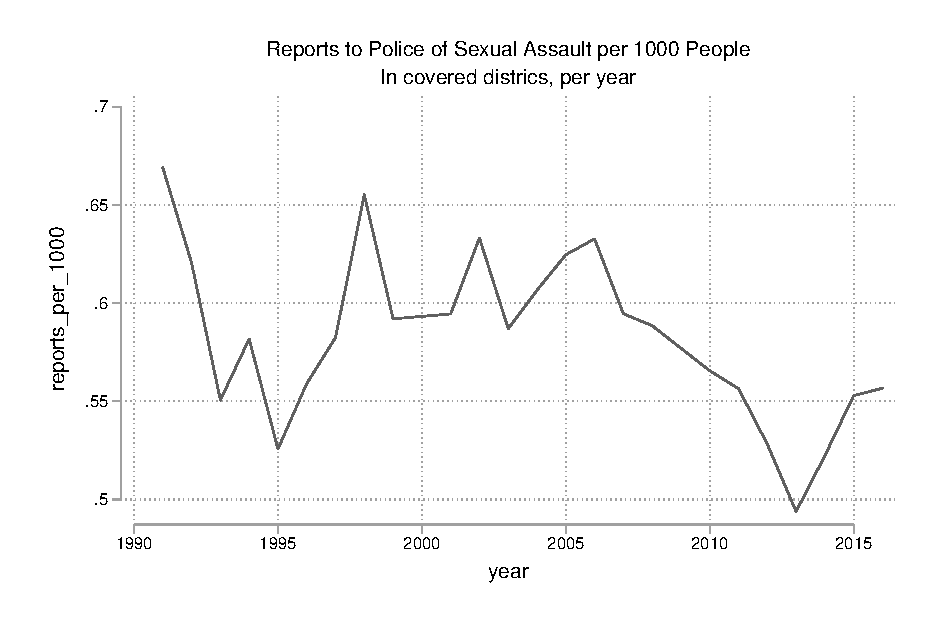
\includegraphics[]{figures/police_yearly_reports.eps}

\caption{Reports to Police per Person, 1991 to 2015}
\end{figure}

\begin{figure}
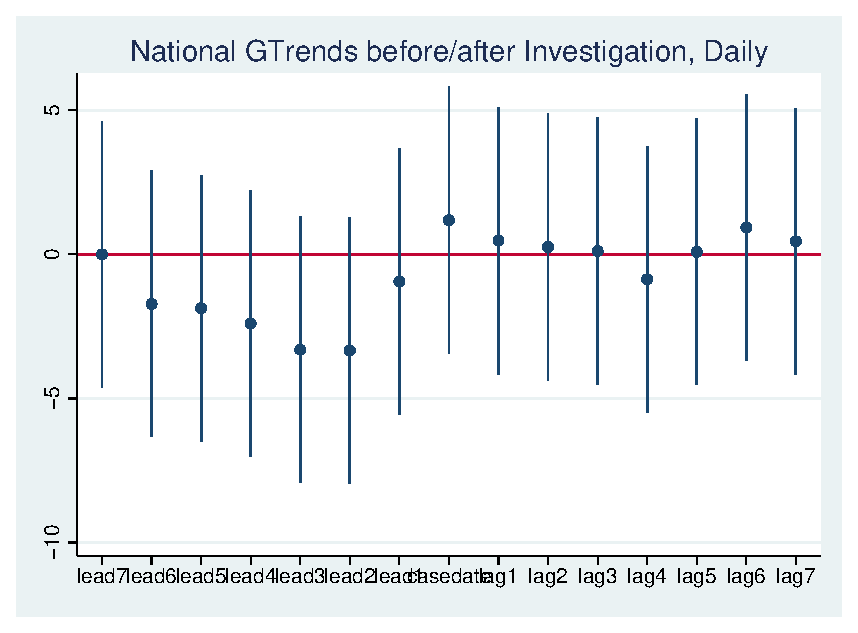
\includegraphics[]{figures/national_trend_cases.eps}

\caption{Daily National Google Trends Before/After T9 Investigation is Opened}
\end{figure}

\begin{figure}
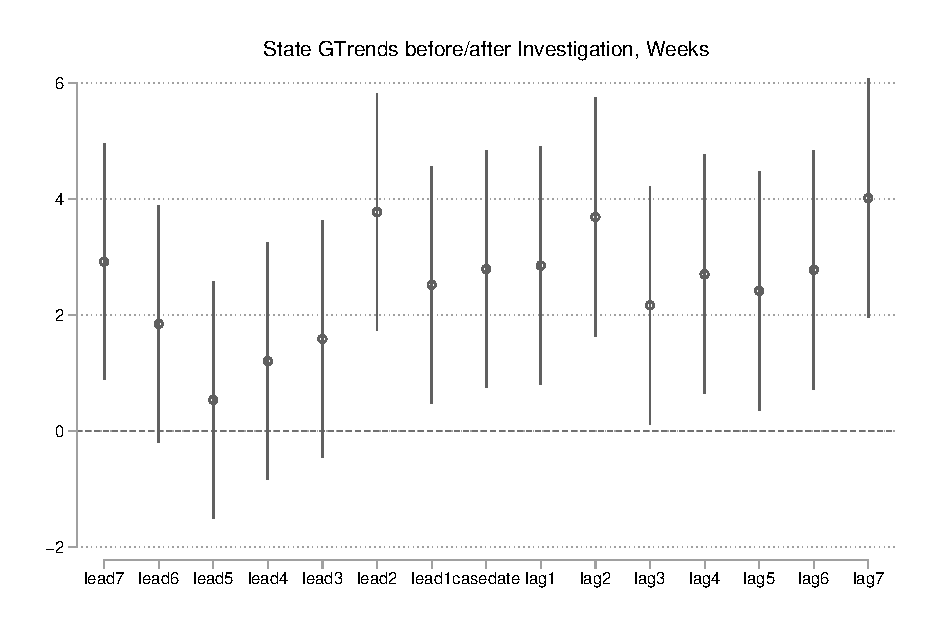
\includegraphics[]{figures/state_trend_cases.eps}

\caption{Weekly State Google Trends Before/After T9 Investigation is Opened}

\end{figure}

\begin{figure}
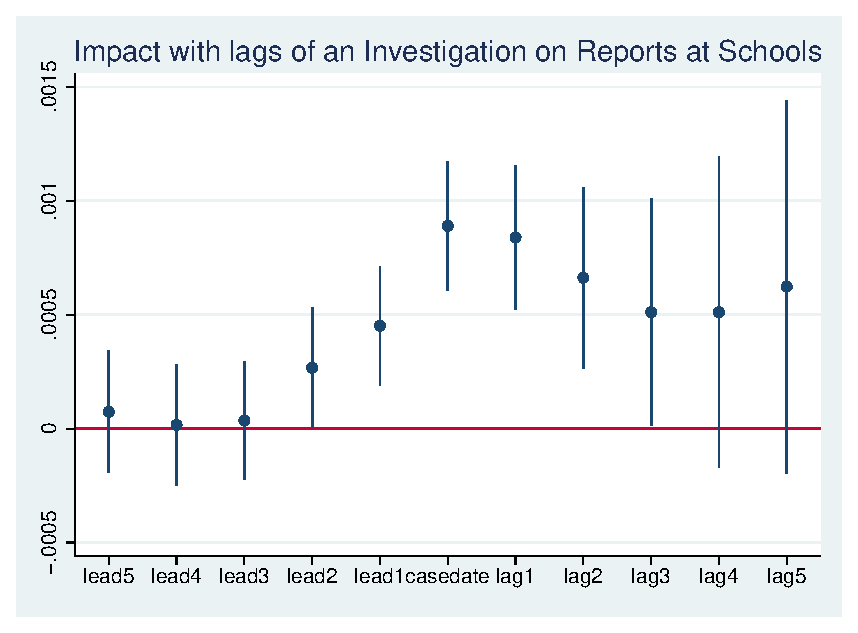
\includegraphics[width=4.9in]{figures/cases_schools_reports_lags.eps}

\caption{Impact of T9 Investigations on Reports at Schools}
\end{figure}

\begin{figure}
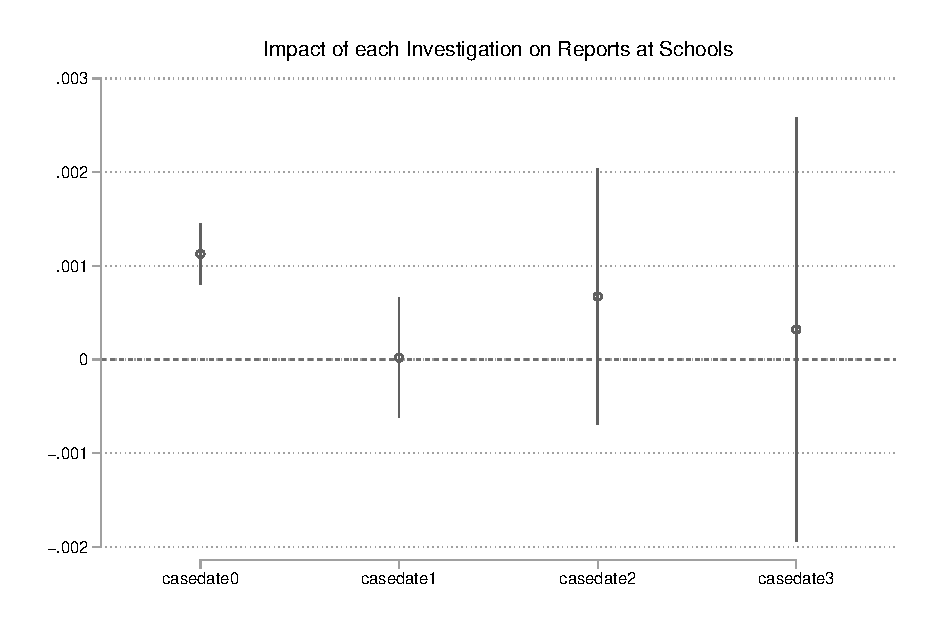
\includegraphics[width=4.9in]{figures/cases_school_reports_numbered.eps}

\caption{Impact of T9 Investigations on Reports at Schools, Numbered}

\end{figure}

\begin{table}
\caption{Reports to Police/Schools in Same County by Year}

{
\def\sym#1{\ifmmode^{#1}\else\(^{#1}\)\fi}
\begin{tabular}{l*{1}{c}}
\hline\hline
            &\multicolumn{1}{c}{(1)}\\
            &\multicolumn{1}{c}{police\_pc}\\
\hline
school\_pc   &      0.0379         \\
            &    (0.0722)         \\
[1em]
\_cons      &    0.000921\sym{***}\\
            & (0.0000333)         \\
\hline
\(N\)       &        1476         \\
adj. \(R^{2}\)&      -0.166         \\
\hline\hline
\multicolumn{2}{l}{\footnotesize Standard errors in parentheses}\\
\multicolumn{2}{l}{\footnotesize \sym{*} \(p<0.05\), \sym{**} \(p<0.01\), \sym{***} \(p<0.001\)}\\
\end{tabular}
}


\end{table}


\begin{table}
\caption{Reports in Schools with Title IX Cases}

{
\def\sym#1{\ifmmode^{#1}\else\(^{#1}\)\fi}
\begin{tabular}{l*{3}{c}}
\hline\hline
            &\multicolumn{1}{c}{(1)}&\multicolumn{1}{c}{(2)}&\multicolumn{1}{c}{(3)}\\
            &\multicolumn{1}{c}{percap}&\multicolumn{1}{c}{percap}&\multicolumn{1}{c}{percap}\\
\hline
lead2       &   0.0000530\sym{*}  &                     &   0.0000530\sym{*}  \\
            & (0.0000207)         &                     & (0.0000207)         \\
[1em]
lead1       &    0.000137\sym{***}&                     &    0.000137\sym{***}\\
            & (0.0000210)         &                     & (0.0000210)         \\
[1em]
yof         &    0.000147\sym{***}&                     &    0.000147\sym{***}\\
            & (0.0000226)         &                     & (0.0000226)         \\
[1em]
lag1        &    0.000218\sym{***}&                     &    0.000218\sym{***}\\
            & (0.0000242)         &                     & (0.0000242)         \\
[1em]
lag2        &    0.000320\sym{***}&                     &    0.000320\sym{***}\\
            & (0.0000275)         &                     & (0.0000275)         \\
[1em]
after\_2011  &                     &    0.000259\sym{***}&    0.000234\sym{***}\\
            &                     & (0.0000115)         & (0.0000115)         \\
[1em]
\_cons      &    0.000123\sym{***}&    0.000123\sym{***}&    0.000123\sym{***}\\
            &(0.00000799)         &(0.00000808)         &(0.00000799)         \\
\hline
\(N\)       &       12887         &       12887         &       12887         \\
adj. \(R^{2}\)&      -0.134         &      -0.160         &      -0.134         \\
\hline\hline
\multicolumn{4}{l}{\footnotesize Standard errors in parentheses}\\
\multicolumn{4}{l}{\footnotesize \sym{*} \(p<0.05\), \sym{**} \(p<0.01\), \sym{***} \(p<0.001\)}\\
\end{tabular}
}


\end{table}

\begin{table}
\caption{Reports in Schools with Title IX Cases, Numbered}

{
\def\sym#1{\ifmmode^{#1}\else\(^{#1}\)\fi}
\begin{tabular}{l*{3}{c}}
\hline\hline
            &\multicolumn{1}{c}{(1)}&\multicolumn{1}{c}{(2)}&\multicolumn{1}{c}{(3)}\\
            &\multicolumn{1}{c}{percap}&\multicolumn{1}{c}{percap}&\multicolumn{1}{c}{percap}\\
\hline
lead10      &    0.000667\sym{***}&                     &    0.000667\sym{***}\\
            &  (0.000155)         &                     &  (0.000155)         \\
[1em]
lead20      &    0.000326\sym{*}  &                     &    0.000326\sym{*}  \\
            &  (0.000151)         &                     &  (0.000151)         \\
[1em]
lead11      &   -0.000122         &                     &   -0.000122         \\
            &  (0.000287)         &                     &  (0.000287)         \\
[1em]
lead21      &  -0.0000845         &                     &  -0.0000845         \\
            &  (0.000278)         &                     &  (0.000278)         \\
[1em]
lead12      &  -0.0000188         &                     &  -0.0000188         \\
            &  (0.000550)         &                     &  (0.000550)         \\
[1em]
lead22      &   0.0000602         &                     &   0.0000602         \\
            &  (0.000510)         &                     &  (0.000510)         \\
[1em]
lead13      &    0.000355         &                     &    0.000355         \\
            &  (0.000893)         &                     &  (0.000893)         \\
[1em]
lead23      &    0.000270         &                     &    0.000270         \\
            &  (0.000764)         &                     &  (0.000764)         \\
[1em]
lead14      &    -0.00144         &                     &    -0.00144         \\
            &   (0.00165)         &                     &   (0.00165)         \\
[1em]
lead24      &   -0.000870         &                     &   -0.000870         \\
            &   (0.00155)         &                     &   (0.00155)         \\
[1em]
lead15      &   -0.000817         &                     &   -0.000817         \\
            &   (0.00317)         &                     &   (0.00317)         \\
[1em]
lead25      &  -0.0000415         &                     &  -0.0000415         \\
            &   (0.00323)         &                     &   (0.00323)         \\
[1em]
lead16      &    0.000608         &                     &    0.000608         \\
            &   (0.00493)         &                     &   (0.00493)         \\
[1em]
lead26      &    0.000687         &                     &    0.000687         \\
            &   (0.00422)         &                     &   (0.00422)         \\
[1em]
casedate0   &     0.00113\sym{***}&                     &     0.00113\sym{***}\\
            &  (0.000166)         &                     &  (0.000166)         \\
[1em]
casedate1   &   0.0000206         &                     &   0.0000206         \\
            &  (0.000328)         &                     &  (0.000328)         \\
[1em]
casedate2   &    0.000672         &                     &    0.000672         \\
            &  (0.000698)         &                     &  (0.000698)         \\
[1em]
casedate3   &    0.000320         &                     &    0.000320         \\
            &   (0.00115)         &                     &   (0.00115)         \\
[1em]
casedate4   &    0.000981         &                     &    0.000981         \\
            &   (0.00175)         &                     &   (0.00175)         \\
[1em]
casedate5   &    -0.00224         &                     &    -0.00224         \\
            &   (0.00411)         &                     &   (0.00411)         \\
[1em]
casedate6   &           0         &                     &           0         \\
            &         (.)         &                     &         (.)         \\
[1em]
lag10       &     0.00112\sym{***}&                     &     0.00112\sym{***}\\
            &  (0.000185)         &                     &  (0.000185)         \\
[1em]
lag20       &    0.000939\sym{***}&                     &    0.000939\sym{***}\\
            &  (0.000228)         &                     &  (0.000228)         \\
[1em]
lag30       &    0.000710\sym{*}  &                     &    0.000710\sym{*}  \\
            &  (0.000279)         &                     &  (0.000279)         \\
[1em]
lag11       &   0.0000343         &                     &   0.0000343         \\
            &  (0.000414)         &                     &  (0.000414)         \\
[1em]
lag21       &   -0.000309         &                     &   -0.000309         \\
            &  (0.000609)         &                     &  (0.000609)         \\
[1em]
lag31       &    0.000742         &                     &    0.000742         \\
            &  (0.000999)         &                     &  (0.000999)         \\
[1em]
lag12       &   -0.000110         &                     &   -0.000110         \\
            &   (0.00104)         &                     &   (0.00104)         \\
[1em]
lag22       &     0.00162         &                     &     0.00162         \\
            &   (0.00207)         &                     &   (0.00207)         \\
[1em]
lag32       &    0.000731         &                     &    0.000731         \\
            &   (0.00351)         &                     &   (0.00351)         \\
[1em]
lag13       &    0.000385         &                     &    0.000385         \\
            &   (0.00175)         &                     &   (0.00175)         \\
[1em]
lag23       &    -0.00174         &                     &    -0.00174         \\
            &   (0.00377)         &                     &   (0.00377)         \\
[1em]
lag33       &    0.000591         &                     &    0.000591         \\
            &   (0.00567)         &                     &   (0.00567)         \\
[1em]
lag14       &     0.00302         &                     &     0.00302         \\
            &   (0.00292)         &                     &   (0.00292)         \\
[1em]
lag24       &     0.00799         &                     &     0.00799         \\
            &   (0.00417)         &                     &   (0.00417)         \\
[1em]
lag34       &           0         &                     &           0         \\
            &         (.)         &                     &         (.)         \\
[1em]
lag15       &           0         &                     &           0         \\
            &         (.)         &                     &         (.)         \\
[1em]
lag25       &           0         &                     &           0         \\
            &         (.)         &                     &         (.)         \\
[1em]
lag35       &           0         &                     &           0         \\
            &         (.)         &                     &         (.)         \\
[1em]
lag16       &           0         &                     &           0         \\
            &         (.)         &                     &         (.)         \\
[1em]
lag26       &           0         &                     &           0         \\
            &         (.)         &                     &         (.)         \\
[1em]
lag36       &           0         &                     &           0         \\
            &         (.)         &                     &         (.)         \\
[1em]
after\_2011  &                     &    0.000313\sym{***}&    0.000276\sym{***}\\
            &                     & (0.0000409)         & (0.0000411)         \\
[1em]
\_cons      &    0.000162\sym{***}&    0.000162\sym{***}&    0.000162\sym{***}\\
            & (0.0000288)         & (0.0000288)         & (0.0000288)         \\
\hline
\(N\)       &       82882         &       82882         &       82882         \\
adj. \(R^{2}\)&      -0.153         &      -0.155         &      -0.153         \\
\hline\hline
\multicolumn{4}{l}{\footnotesize Standard errors in parentheses}\\
\multicolumn{4}{l}{\footnotesize \sym{*} \(p<0.05\), \sym{**} \(p<0.01\), \sym{***} \(p<0.001\)}\\
\end{tabular}
}


\end{table}


\begin{table}
\caption{Reports to Schools in same County as Schools with Title IX Cases}

{
\def\sym#1{\ifmmode^{#1}\else\(^{#1}\)\fi}
\begin{tabular}{l*{1}{c}}
\hline\hline
            &\multicolumn{1}{c}{(1)}\\
            &\multicolumn{1}{c}{school\_pc}\\
\hline
lead2       &  -0.0000329         \\
            & (0.0000234)         \\
[1em]
lead1       &  -0.0000432         \\
            & (0.0000234)         \\
[1em]
yof         &  -0.0000475         \\
            & (0.0000249)         \\
[1em]
lag1        &  -0.0000575\sym{*}  \\
            & (0.0000260)         \\
[1em]
lag2        &  -0.0000465         \\
            & (0.0000288)         \\
[1em]
\_cons      &    0.000106\sym{***}\\
            &(0.00000950)         \\
\hline
\(N\)       &        6309         \\
adj. \(R^{2}\)&       0.022         \\
\hline\hline
\multicolumn{2}{l}{\footnotesize Standard errors in parentheses}\\
\multicolumn{2}{l}{\footnotesize \sym{*} \(p<0.05\), \sym{**} \(p<0.01\), \sym{***} \(p<0.001\)}\\
\end{tabular}
}

\end{table}

\begin{table}
\caption{Reports to Police in same County as Schools with Title IX Cases}

{
\def\sym#1{\ifmmode^{#1}\else\(^{#1}\)\fi}
\begin{tabular}{l*{1}{c}}
\hline\hline
            &\multicolumn{1}{c}{(1)}\\
            &\multicolumn{1}{c}{county\_pc}\\
\hline
lead2       &  -0.0000932         \\
            &  (0.000262)         \\
[1em]
lead1       &  -0.0000685         \\
            &  (0.000333)         \\
[1em]
yof         & 0.000000416         \\
            &  (0.000390)         \\
[1em]
lag1        &    0.000118         \\
            &  (0.000432)         \\
[1em]
lag2        &    0.000154         \\
            &  (0.000587)         \\
[1em]
\_cons      &    0.000664\sym{***}\\
            &  (0.000143)         \\
\hline
\(N\)       &       18094         \\
adj. \(R^{2}\)&      -0.078         \\
\hline\hline
\multicolumn{2}{l}{\footnotesize Standard errors in parentheses}\\
\multicolumn{2}{l}{\footnotesize \sym{*} \(p<0.05\), \sym{**} \(p<0.01\), \sym{***} \(p<0.001\)}\\
\end{tabular}
}


%\begin{tablenotes}
%Table notes environment without optional leadin.
%\end{tablenotes}
%\begin{tablenotes}[Source]
%Table notes environment with optional leadin (Source, in this case).
%\end{tablenotes}
\end{table}



\begin{table}
\caption{Reports to Police vs Trends, Daily}

{
\def\sym#1{\ifmmode^{#1}\else\(^{#1}\)\fi}
\begin{tabular}{l*{4}{c}}
\hline\hline
            &\multicolumn{1}{c}{(1)}&\multicolumn{1}{c}{(2)}&\multicolumn{1}{c}{(3)}&\multicolumn{1}{c}{(4)}\\
            &\multicolumn{1}{c}{log\_rape}&\multicolumn{1}{c}{rape}&\multicolumn{1}{c}{rape}&\multicolumn{1}{c}{rape}\\
\hline
lag7        &     -0.0439\sym{**} &    -0.00995         &     -0.0440         &     -0.0418         \\
            &    (0.0139)         &   (0.00642)         &    (0.0327)         &    (0.0326)         \\
[1em]
lag6        &     -0.0148         &     0.00815         &     -0.0184         &     -0.0185         \\
            &    (0.0145)         &   (0.00771)         &    (0.0371)         &    (0.0370)         \\
[1em]
lag5        &      0.0126         &    -0.00661         &      0.0512         &      0.0517         \\
            &    (0.0146)         &   (0.00769)         &    (0.0372)         &    (0.0371)         \\
[1em]
lag4        &     0.00395         &    -0.00221         &     -0.0193         &     -0.0208         \\
            &    (0.0147)         &   (0.00773)         &    (0.0372)         &    (0.0371)         \\
[1em]
lag3        &     0.00630         &     0.00989         &   -0.000318         &    0.000166         \\
            &    (0.0147)         &   (0.00774)         &    (0.0372)         &    (0.0371)         \\
[1em]
lag2        &    -0.00317         &     0.00575         &      0.0149         &      0.0143         \\
            &    (0.0147)         &   (0.00780)         &    (0.0373)         &    (0.0372)         \\
[1em]
lag1        &      0.0271         &     0.00104         &      0.0545         &      0.0534         \\
            &    (0.0147)         &   (0.00779)         &    (0.0373)         &    (0.0371)         \\
[1em]
trend       &    -0.00690         &     -0.0107         &     -0.0686         &     -0.0668         \\
            &    (0.0147)         &   (0.00782)         &    (0.0372)         &    (0.0371)         \\
[1em]
lead1       &      0.0549\sym{***}&     0.00559         &      0.0916\sym{*}  &      0.0911\sym{*}  \\
            &    (0.0147)         &   (0.00777)         &    (0.0373)         &    (0.0372)         \\
[1em]
lead2       &     -0.0101         &   -0.000530         &     -0.0527         &     -0.0529         \\
            &    (0.0147)         &   (0.00766)         &    (0.0372)         &    (0.0371)         \\
[1em]
lead3       &     -0.0120         &     0.00445         &     -0.0228         &     -0.0230         \\
            &    (0.0147)         &   (0.00766)         &    (0.0372)         &    (0.0371)         \\
[1em]
lead4       &    -0.00293         &    -0.00979         &     -0.0198         &     -0.0193         \\
            &    (0.0147)         &   (0.00760)         &    (0.0372)         &    (0.0371)         \\
[1em]
lead5       &      0.0226         &    -0.00733         &      0.0123         &      0.0128         \\
            &    (0.0147)         &   (0.00755)         &    (0.0372)         &    (0.0371)         \\
[1em]
lead6       &      0.0174         &   -0.000961         &      0.0221         &      0.0213         \\
            &    (0.0145)         &   (0.00751)         &    (0.0371)         &    (0.0369)         \\
[1em]
lead7       &     -0.0160         &     0.00544         &      0.0155         &      0.0155         \\
            &    (0.0139)         &   (0.00632)         &    (0.0327)         &    (0.0326)         \\
[1em]
\_cons      &       4.649\sym{***}&       38.11\sym{***}&       149.2\sym{***}&       147.6\sym{***}\\
            &    (0.0867)         &     (1.140)         &     (5.015)         &     (4.999)         \\
\hline
\(N\)       &        3274         &        1387         &        3274         &        3274         \\
adj. \(R^{2}\)&       0.280         &       0.831         &       0.210         &       0.211         \\
\hline\hline
\multicolumn{5}{l}{\footnotesize Standard errors in parentheses}\\
\multicolumn{5}{l}{\footnotesize \sym{*} \(p<0.05\), \sym{**} \(p<0.01\), \sym{***} \(p<0.001\)}\\
\end{tabular}
}

\end{table}


\begin{table}
\caption{Reports to Police vs Trends, Week by State}

{
\def\sym#1{\ifmmode^{#1}\else\(^{#1}\)\fi}
\begin{tabular}{l*{1}{c}}
\hline\hline
            &\multicolumn{1}{c}{(1)}\\
            &\multicolumn{1}{c}{rape}\\
\hline
lead7       &      0.0239         \\
            &    (0.0149)         \\
[1em]
lead6       &      0.0246         \\
            &    (0.0149)         \\
[1em]
lead5       &      0.0191         \\
            &    (0.0150)         \\
[1em]
lead4       &      0.0164         \\
            &    (0.0150)         \\
[1em]
lead3       &      0.0214         \\
            &    (0.0150)         \\
[1em]
lead2       &      0.0213         \\
            &    (0.0150)         \\
[1em]
lead1       &      0.0219         \\
            &    (0.0150)         \\
[1em]
trend       &      0.0176         \\
            &    (0.0150)         \\
[1em]
lag1        &      0.0137         \\
            &    (0.0149)         \\
[1em]
lag2        &     0.00802         \\
            &    (0.0149)         \\
[1em]
lag3        &      0.0273         \\
            &    (0.0148)         \\
[1em]
lag4        &      0.0206         \\
            &    (0.0148)         \\
[1em]
lag5        &      0.0300\sym{*}  \\
            &    (0.0148)         \\
[1em]
lag6        &      0.0246         \\
            &    (0.0147)         \\
[1em]
lag7        &      0.0279         \\
            &    (0.0147)         \\
[1em]
\_cons      &       20.05\sym{***}\\
            &     (2.223)         \\
\hline
\(N\)       &       12863         \\
adj. \(R^{2}\)&                     \\
\hline\hline
\multicolumn{2}{l}{\footnotesize Standard errors in parentheses}\\
\multicolumn{2}{l}{\footnotesize \sym{*} \(p<0.05\), \sym{**} \(p<0.01\), \sym{***} \(p<0.001\)}\\
\end{tabular}
}

\end{table}


\begin{table}
\caption{Reports to Police before/after High Trends, Daily}

{
\def\sym#1{\ifmmode^{#1}\else\(^{#1}\)\fi}
\begin{tabular}{l*{5}{c}}
\hline\hline
            &\multicolumn{1}{c}{(1)}&\multicolumn{1}{c}{(2)}&\multicolumn{1}{c}{(3)}&\multicolumn{1}{c}{(4)}&\multicolumn{1}{c}{(5)}\\
            &\multicolumn{1}{c}{rape}&\multicolumn{1}{c}{rape}&\multicolumn{1}{c}{rape}&\multicolumn{1}{c}{rape}&\multicolumn{1}{c}{rape}\\
\hline
lead7       &      -0.404         &      -2.653         &      -0.206         &       5.573         &      -0.760         \\
            &     (1.542)         &     (2.012)         &     (3.296)         &     (6.209)         &     (12.12)         \\
[1em]
lead6       &       0.584         &       1.043         &      -0.186         &       0.243         &       10.01         \\
            &     (1.559)         &     (2.058)         &     (3.382)         &     (6.644)         &     (12.23)         \\
[1em]
lead5       &       3.097\sym{*}  &       0.850         &      -1.201         &      -7.551         &      -2.940         \\
            &     (1.558)         &     (2.062)         &     (3.388)         &     (6.732)         &     (13.27)         \\
[1em]
lead4       &      -1.683         &      0.0585         &      -1.669         &       5.939         &      -9.904         \\
            &     (1.556)         &     (2.060)         &     (3.381)         &     (6.747)         &     (13.29)         \\
[1em]
lead3       &      -0.578         &      -2.865         &      -6.037         &      -4.926         &      -4.909         \\
            &     (1.556)         &     (2.063)         &     (3.383)         &     (6.755)         &     (13.29)         \\
[1em]
lead2       &      -1.866         &       0.656         &       0.793         &      -0.545         &      -7.530         \\
            &     (1.553)         &     (2.059)         &     (3.394)         &     (6.754)         &     (13.29)         \\
[1em]
lead1       &       2.302         &       4.698\sym{*}  &       8.910\sym{**} &       1.960         &       13.65         \\
            &     (1.558)         &     (2.065)         &     (3.405)         &     (6.760)         &     (13.37)         \\
[1em]
dateofhigh  &       0.307         &       0.900         &       1.220         &       7.871         &       13.93         \\
            &     (1.562)         &     (2.078)         &     (3.430)         &     (6.777)         &     (13.29)         \\
[1em]
lag1        &       0.550         &       0.687         &       1.399         &      -4.199         &      -8.983         \\
            &     (1.556)         &     (2.071)         &     (3.413)         &     (6.756)         &     (13.30)         \\
[1em]
lag2        &      -2.189         &      -0.728         &       4.964         &       3.492         &      -7.793         \\
            &     (1.557)         &     (2.062)         &     (3.400)         &     (6.748)         &     (13.29)         \\
[1em]
lag3        &       1.965         &       1.623         &      -2.449         &      -0.707         &      -7.059         \\
            &     (1.556)         &     (2.063)         &     (3.383)         &     (6.754)         &     (13.29)         \\
[1em]
lag4        &      -0.561         &      -0.955         &      -1.922         &      -4.990         &      -7.340         \\
            &     (1.556)         &     (2.067)         &     (3.382)         &     (6.748)         &     (13.29)         \\
[1em]
lag5        &       0.861         &      -0.506         &      -3.359         &      -3.124         &      -6.002         \\
            &     (1.553)         &     (2.065)         &     (3.385)         &     (6.750)         &     (13.29)         \\
[1em]
lag6        &      -1.537         &      -0.351         &      -0.657         &      -0.675         &       7.951         \\
            &     (1.558)         &     (2.061)         &     (3.387)         &     (6.731)         &     (13.35)         \\
[1em]
lag7        &      -0.529         &       1.645         &       4.737         &      -0.869         &      -4.123         \\
            &     (1.536)         &     (2.025)         &     (3.325)         &     (6.371)         &     (13.12)         \\
[1em]
\_cons      &       150.5\sym{***}&       151.4\sym{***}&       151.9\sym{***}&       150.7\sym{***}&       150.7\sym{***}\\
            &     (5.141)         &     (5.058)         &     (5.023)         &     (5.025)         &     (5.019)         \\
\hline
\(N\)       &        2908         &        2908         &        2908         &        2908         &        2908         \\
adj. \(R^{2}\)&       0.170         &       0.170         &       0.173         &       0.168         &       0.168         \\
\hline\hline
\multicolumn{6}{l}{\footnotesize Standard errors in parentheses}\\
\multicolumn{6}{l}{\footnotesize \sym{*} \(p<0.05\), \sym{**} \(p<0.01\), \sym{***} \(p<0.001\)}\\
\end{tabular}
}

\end{table}


\begin{table}
\caption{Reports to Police before/after High Trends, Week by State}

{
\def\sym#1{\ifmmode^{#1}\else\(^{#1}\)\fi}
\begin{tabular}{l*{5}{c}}
\hline\hline
            &\multicolumn{1}{c}{(1)}&\multicolumn{1}{c}{(2)}&\multicolumn{1}{c}{(3)}&\multicolumn{1}{c}{(4)}&\multicolumn{1}{c}{(5)}\\
            &\multicolumn{1}{c}{rape}&\multicolumn{1}{c}{rape}&\multicolumn{1}{c}{rape}&\multicolumn{1}{c}{rape}&\multicolumn{1}{c}{rape}\\
\hline
lead7       &       0.384         &       0.201         &       0.346         &       5.125         &       3.313         \\
            &     (0.906)         &     (1.704)         &     (3.337)         &     (8.188)         &     (12.50)         \\
[1em]
lead6       &       0.290         &      -0.829         &       0.705         &       3.642         &       0.564         \\
            &     (0.910)         &     (1.709)         &     (3.340)         &     (8.173)         &     (12.32)         \\
[1em]
lead5       &       0.436         &      -0.291         &       1.471         &       5.546         &       3.689         \\
            &     (0.911)         &     (1.707)         &     (3.327)         &     (8.257)         &     (12.32)         \\
[1em]
lead4       &       0.570         &      -0.166         &      -0.133         &       0.509         &       1.355         \\
            &     (0.913)         &     (1.709)         &     (3.309)         &     (8.583)         &     (12.32)         \\
[1em]
lead3       &       0.212         &      0.0278         &      -1.023         &      -1.248         &      -0.802         \\
            &     (0.913)         &     (1.706)         &     (3.271)         &     (8.586)         &     (12.32)         \\
[1em]
lead2       &       0.143         &       0.393         &     -0.0441         &       0.700         &       3.608         \\
            &     (0.913)         &     (1.707)         &     (3.272)         &     (8.594)         &     (12.32)         \\
[1em]
lead1       &       0.345         &       0.114         &      -0.251         &       0.532         &       3.186         \\
            &     (0.912)         &     (1.703)         &     (3.252)         &     (8.593)         &     (12.32)         \\
[1em]
dateofhigh  &       0.288         &       0.456         &      -0.745         &       0.144         &       1.310         \\
            &     (0.912)         &     (1.708)         &     (3.252)         &     (8.593)         &     (12.32)         \\
[1em]
lag1        &      -0.100         &      -0.495         &      -0.589         &       1.803         &       2.761         \\
            &     (0.912)         &     (1.709)         &     (3.233)         &     (8.593)         &     (12.32)         \\
[1em]
lag2        &      -0.279         &      -0.350         &      -0.560         &       1.377         &       0.389         \\
            &     (0.911)         &     (1.715)         &     (3.272)         &     (8.593)         &     (12.32)         \\
[1em]
lag3        &       0.711         &       0.267         &      -0.110         &       1.717         &       4.543         \\
            &     (0.908)         &     (1.712)         &     (3.270)         &     (8.593)         &     (12.32)         \\
[1em]
lag4        &       0.224         &       0.369         &      -0.733         &      -1.409         &       0.667         \\
            &     (0.906)         &     (1.709)         &     (3.269)         &     (8.590)         &     (12.32)         \\
[1em]
lag5        &       0.987         &       0.772         &       2.256         &      -2.033         &      -3.339         \\
            &     (0.906)         &     (1.712)         &     (3.267)         &     (8.591)         &     (12.32)         \\
[1em]
lag6        &       0.120         &      -0.168         &     -0.0194         &       0.289         &       3.607         \\
            &     (0.903)         &     (1.708)         &     (3.244)         &     (8.489)         &     (12.32)         \\
[1em]
lag7        &       0.224         &      -0.177         &      -0.817         &      -2.176         &       0.129         \\
            &     (0.898)         &     (1.706)         &     (3.259)         &     (8.512)         &     (12.50)         \\
[1em]
\_cons      &       26.13\sym{***}&       26.73\sym{***}&       26.72\sym{***}&       26.72\sym{***}&       26.74\sym{***}\\
            &     (2.209)         &     (2.201)         &     (2.200)         &     (2.198)         &     (2.198)         \\
\hline
\(N\)       &       12863         &       12863         &       12863         &       12863         &       12863         \\
adj. \(R^{2}\)&       0.002         &       0.002         &       0.002         &       0.002         &       0.002         \\
\hline\hline
\multicolumn{6}{l}{\footnotesize Standard errors in parentheses}\\
\multicolumn{6}{l}{\footnotesize \sym{*} \(p<0.05\), \sym{**} \(p<0.01\), \sym{***} \(p<0.001\)}\\
\end{tabular}
}

\end{table}


\end{document}

